\documentclass[unicode]{beamer}
\usepackage[T2A]{fontenc}
\usepackage[utf8]{inputenc}
\usepackage[russian]{babel}
\usepackage{cmap}
\usepackage{amssymb,amsfonts,amsmath,mathtext}
\usepackage{beamerthemesplit,graphicx}
% XeTeX packages
\usepackage[cm-default]{fontspec} % or install lmodern and remove cm-default opt
\usepackage{xunicode} % some extra unicode support
\usepackage{xltxtra} % \XeLaTeX macro
\defaultfontfeatures{Scale=MatchLowercase,Mapping=tex-text}
% Setting default fonts
\setromanfont{Charis SIL}
\setsansfont{Charis SIL}
\setmonofont{Charis SIL}

\usepackage{geometry} % Меняем поля страницы
\geometry{left=3mm}% левое поле — не менее 20 мм
\geometry{right=3mm}% правое поле — не менее 10 мм
\geometry{top=0cm}% верхнее поле — не менее 15 мм
\geometry{bottom=0cm}% нижнее поле — не менее 20 мм
\usetheme{Warsaw}
\setbeamerfont{institute}{size=\normalsize}
\graphicspath{{images/}}

\title[Разработка сетевой архитектуры в проекте HiveMind]{
Разработка сетевой архитектуры для редактора диаграмм связей HiveMind
}
\author[Кандауров О.\,В.]{Кандауров Олег Владимирович}
\institute{
Научный руководитель: ст. преподаватель Парамонов~И.\,В.
}

\date{}

\begin{document}
\maketitle
\large


\begin{frame}
\transwipe[direction=90]
\frametitle{Диаграммы связей}
\begin{figure}[h!] 
\centering
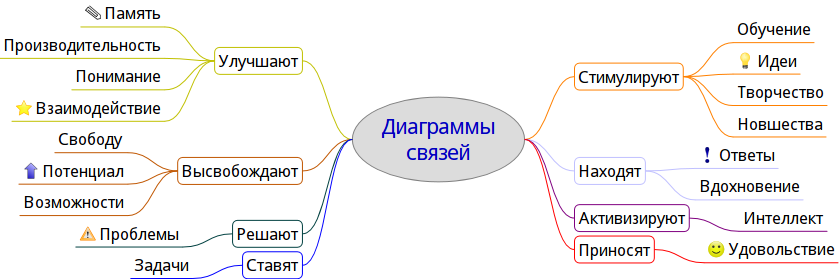
\includegraphics[width=\linewidth]{mindmap} 
\end{figure}
\end{frame}


\begin{frame}
\transwipe[direction=90]
\frametitle{Проект HiveMind}
\begin{figure}[h!]
\begin{minipage}[h]{0.45\linewidth}
\center{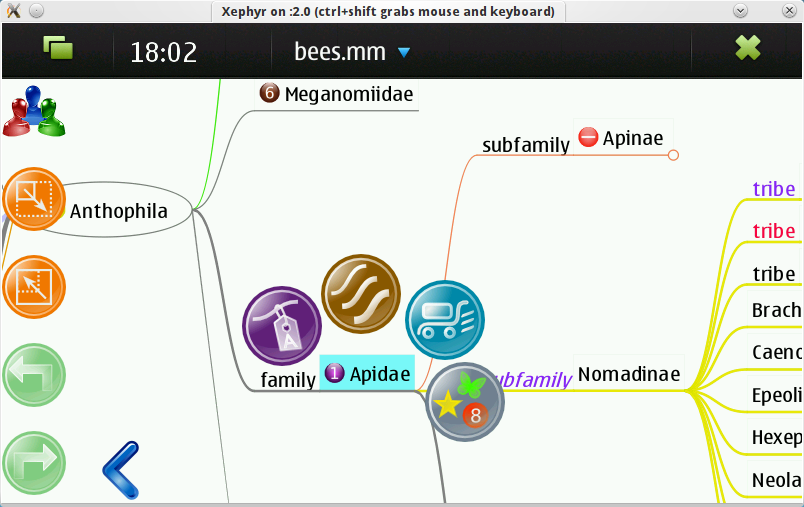
\includegraphics[width=1\linewidth]{hivemind-maemo}}
\end{minipage}
\hfill
\begin{minipage}[h]{0.45\linewidth}
\center{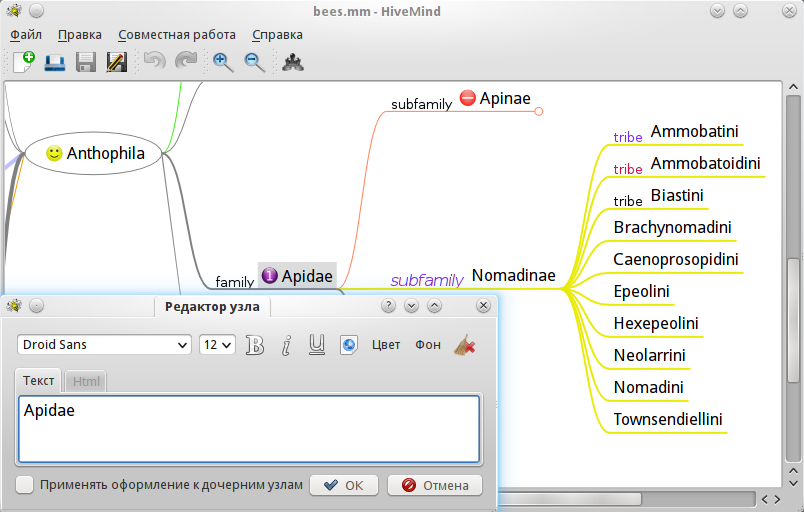
\includegraphics[width=1\linewidth]{hivemind-linux}}
\end{minipage}
\vfill
\begin{minipage}[h]{0.45\linewidth}
\center{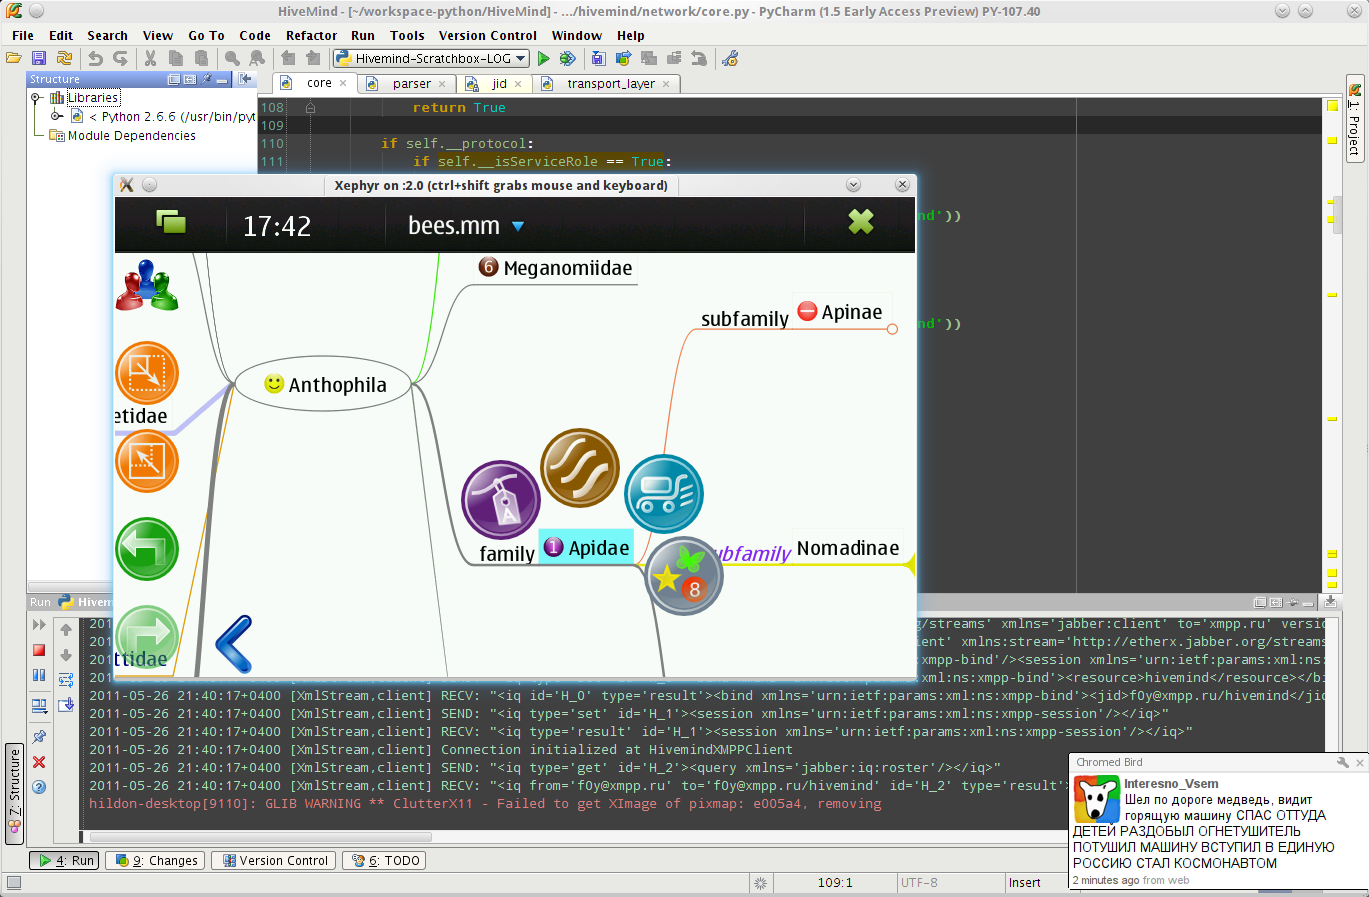
\includegraphics[width=1\linewidth]{hivemind-meego}}
\end{minipage}
\hfill
\begin{minipage}[h]{0.45\linewidth}
\center{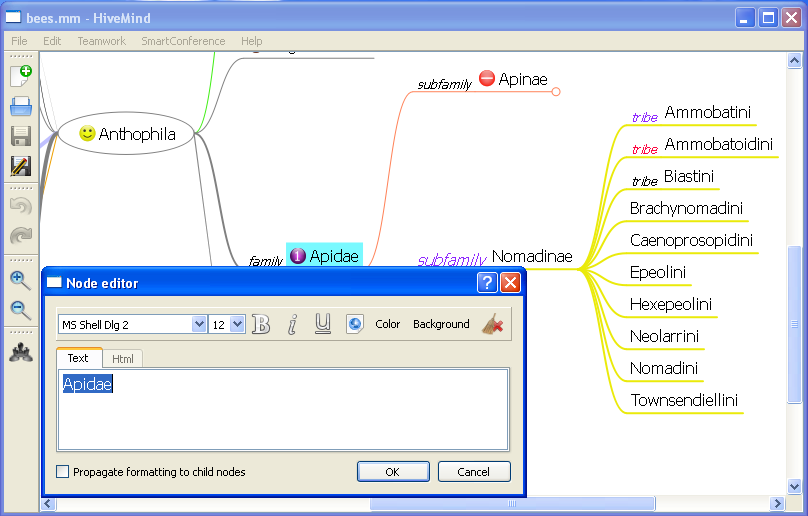
\includegraphics[width=1\linewidth]{hivemind-windows}}
\end{minipage}
\end{figure}
\end{frame}


\begin{frame}
\transwipe[direction=90]
\frametitle{Постановка задачи}
\begin{block}{Реализовать возможность совместного редактирования диаграмм связей
в проекте HiveMind}
  \begin{itemize}
    \item Выбрать технологию промежуточного слоя и средства для работы с ним
    \item Разработать гибкую сетевую архитектуру для совместного редактирования
    \item Реализовать разработанную архитектуру в приложении HiveMind
  \end{itemize}
\end{block}
\end{frame}

\begin{frame}
\transwipe[direction=90]
\frametitle{Сетевая архитектура}
\begin{figure}[h!] 
\centering
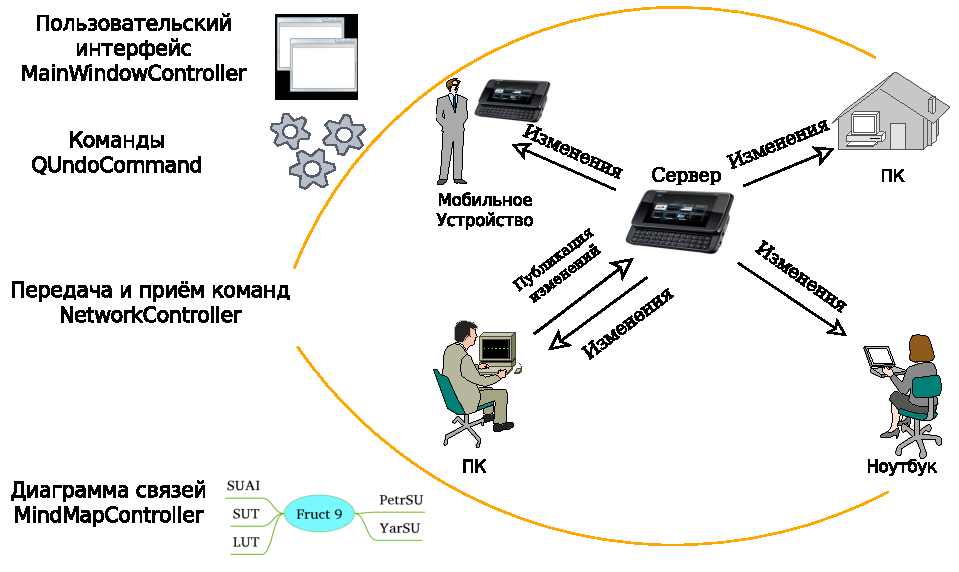
\includegraphics[width=\linewidth]{application-layers-improved} 
\end{figure}
\end{frame}


\begin{frame}
\transwipe[direction=90]
\frametitle{Реализация}
\begin{figure}[h!] 
\centering
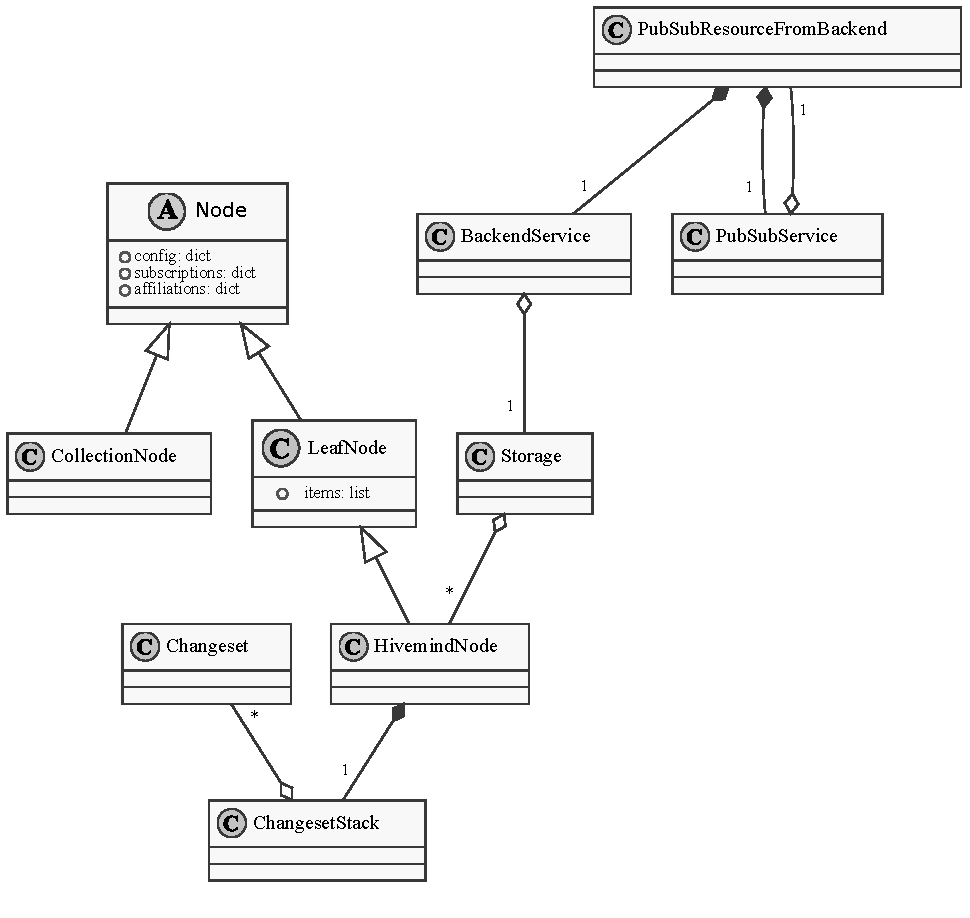
\includegraphics[scale=0.65]{idavoll-classes} 
\end{figure}
\end{frame}

\begin{frame}
\transwipe[direction=90]
\frametitle{Результаты работы}
\begin{itemize}
  \item Разработана сетевая архитектура, позволяющая выполнять совместное
  редактирование документов
  \item Архитектура успешно реализована в приложении HiveMind
  \item Реализованный функционал позволяет эффективно выполнять совместное
  редактирование диаграмм связей на всех целевых платформах
  \item Результаты работы представлены на 9-й конференции международной
  программы открытых инноваций FRUCT
\end{itemize}
\end{frame}
\end{document}